\section{Tool Implementation}\label{tool-implementation}

Below is the definition of the FoldFeature superclass --- all features
created using Foldlings can override these methods to provide specific
functionality. This structure holds properties common to all features,
such as a list of edges and parent-child relationships between features.
It also contains several functions that allow the other classes to
modify the feature and sketch. For further discussion of the FoldFeature
data structure, see \textbf{\textgreater{}\textgreater{}TODO REF}.

\small
\singlespacing 

\begin{pygmented}{swift}
var horizontalFolds:[Edge] = [] //list of horizontal folds
var featureEdges:[Edge]?        //edges in a feature
var children:[FoldFeature] = [] // children of feature
var drivingFold:Edge? // driving fold of feature
var parent:FoldFeature? // parent of feature
var startPoint:CGPoint?
var endPoint:CGPoint? // start and end touch points

/// splits an edge around the current feature
func splitFoldByOcclusion(edge:Edge) -> [Edge]
{
//by default, return edge whole
return [edge]
}
/// features are leaves if they don't have children
func isLeaf() -> Bool
{
return children.count == 0
}
/// options or modifications that can be made to the current feature
func tapOptions() -> [FeatureOption]?
{
  return [FeatureOption.PrintPlanes, FeatureOption.PrintEdges,
  FeatureOption.ColorPlaneEdges, FeatureOption.PrintSinglePlane]
}
/// whether a feature is drawn over a fold, determines whether 
/// a fold can be the driving fold for a feature
  func featureSpansFold(fold:Edge)->Bool
{
  return false
}
/// returns and calculates planes in a feature
func getFeaturePlanes()-> [Plane]{
  return featurePlanes
}
/// whether a feature contains a point
/// needs to be overridden by subclasses
func containsPoint(point:CGPoint) -> Bool{
  return self.boundingBox()?.contains(point) ?? false
}
\end{pygmented}

\doublespacing
\normalsize

Of these functions, the most complex are \emph{featureSpansFold} and
\emph{splitFoldByOcclusion}. \emph{FeatureSpansFold} is the test to find
the driving for a feature ---~i.e.~the fold over which a feature is
drawn. The implementation of this function varies by feature, but the
general algorithm is as follow:

\begin{enumerate}
\def\labelenumi{\arabic{enumi})}
\itemsep1pt\parskip0pt\parsep0pt
\item
  Test for intersections between the shape's outer path and the given
  fold.

  \begin{enumerate}
  \def\labelenumii{(\alph{enumii})}
  \itemsep1pt\parskip0pt\parsep0pt
  \item
    If an even number of intersection points are found, return true,
    otherwise, return false. Fold features with multiple potential
    driving folds are consider invalid.
  \end{enumerate}
\end{enumerate}

\emph{SplitFoldByOcclusion} takes as a fold as its input, typically the
driving fold for the feature. The function splits the given fold into
multiple pieces, removing sections of the edge that would lie inside the
bounds of the feature on which the method is called.

\begin{figure}[htbp]
\centering
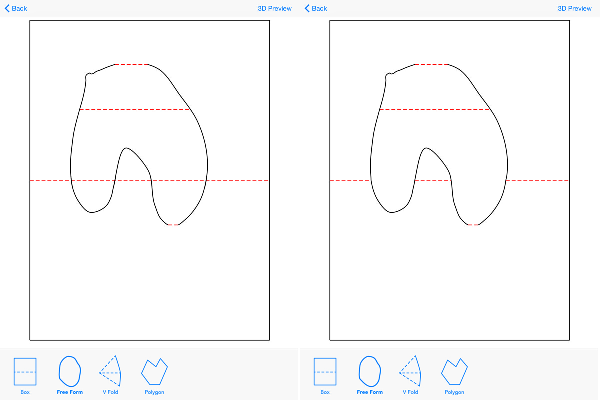
\includegraphics{figures/41_Tech_Tool_Implementation/splitfoldbyOcclusionBeforeAfter.pdf}
\caption{Left: a freeform shape before performing
\emph{SplitFoldByOcclusion}. Right: a freeform feature after performing
\emph{SplitFoldByOcclusion}.}
\end{figure}

\subsection{Box Fold}\label{box-fold}

We can analytically determine intersection points for box folds, which
makes testing for fold spanning and other operations very fast. We
dynamically update edges for feature (including the middle fold), as the
user drags out the box. Box folds are the only feature for which we can
display a live preview of the middle fold, as a result of the simple
intersection tests.

\subsubsection{FreeForm}\label{freeform}

A freeform shape consists of a series of interpolation points
---~through which we construct a curve using the Catmull-Rom algorithm.
\textbf{\textgreater{}\textgreater{}TODO:CITE} We capture interpolation
points as a function of touch velocity. That is, when the user draws
more quickly, we capture more interpolation points closer together. This
allows us to capture the entire drawing with a similar level of detail
throughout, and correct for the gesture recognizer sending relatively
more frequent updates when the touch is moving more slowly.

However, the catmull-Rom algorithm only draws a full path when the start
and end points of the curve are coincident, so we manually construct
straight line segments to and from the touch start and end points for
unclosed freeform shapes. We use an alpha value of 1.0, which we found
to be the closest to the intended touch shape through informal user
studies.

\paragraph{Truncation}\label{truncation}

\begin{figure}[htbp]
\centering
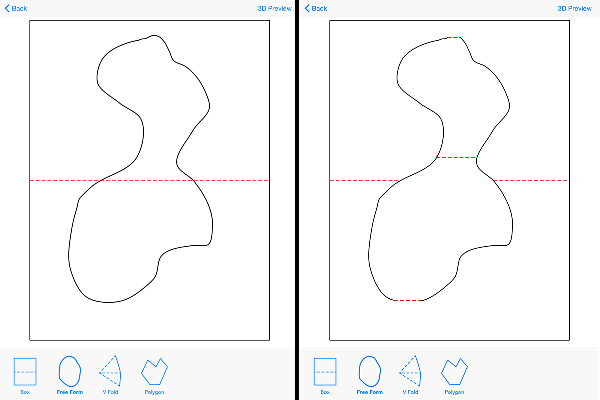
\includegraphics{figures/41_Tech_Tool_Implementation/truncationBeforeAfter.pdf}
\caption{Left: A freeform feature before truncation. Right: A freeform
feature after truncation}
\end{figure}

Truncation is the process of converting a closed free-form shape into a
valid feature with a driving fold. To truncate a shape, we first find
locations for top and bottom folds that will yield folds longer than the
minimum edge length. Then, we split the existing path at those
intersection points, and remove paths that lie outside the top and
bottom folds of the new shape. Thus, we ``truncate'' the shape, adding
horizontal folds and trimming edges that lie outside the new shape.
Finally, we place the middle fold as described by the geometric
constraints in chapter, page\textbf{\textgreater{}\textgreater{}TODO:
REF}. If the user desires different truncation positions, they can drag
folds after the feature is added to the sketch.

\begin{algorithm}[H]

\KwData{\textit{path}, the bezier path for the freeform shape}

\KwResult{edges for truncated shape}

create \textit{scanline} at top of bounding box for \textit{feature}

\While{\textit{scanline} above bottom of \textit{feature}}{

\textit{intercepts} $\leftarrow$ intersection points between \textit{scanline} and \textit{path}

\If{\textit{intercepts} not nil  and distance between\textit{ intercepts} $>$ min edge length}{

    \textit{fragments} $\leftarrow$ \textit{path} split by \textit{intercepts}
    
    \ForEach{\textit{fragment} in \textit{fragments}}{
    
    \If{\textit{fragment} center is above top fold or below bottom fold}{
    
    remove \textit{fragment} from \textit{fragments}
    
    }
    
    }
    
\bf{break}

}

translate \textit{scanline} down

}
 
repeat \textit{scanline} operation from bottom to find bottom fold
    
calculate middle fold position
    
\textit{folds} $\leftarrow$ top, middle, and bottom folds
    
\Return{\textit{folds} + \textit{fragments}}  

\caption{Truncation}
\end{algorithm}

This algorithm depends on the ability to calculate intersections between
bezier paths. We use a bitmap approximation of the intersection point
between bezier paths, because calculating intersections between
arbitrary curves is computationally more expensive. We use the
\emph{ANPathIntersection} library for intersections, which draws the two
paths into a buffer, and then finds points where both paths have pixels
filled (\citet{ANPathIntersection}). This fast approximation allows us
to perform the many intersection tests required for truncation quickly,
minimizing the delay after creating a feature.

After finding the intersection points, we split the existing path at the
intersection points. The freeform shape's path is composed of many cubic
bezier curves. In order to split the path, we must first find the
closest cubic bezier curve to the intersection point, and then find a
value, \(t\), that gives interpolated position at the intersection
point. First, we iterate through all bezier segments in the path,
comparing representative points to find the closest curved segment to
the intersection point. Within that segment, we recursively subdivide
the curve to find a \(t\) value very close to the intersection point
(\citet{phillips1997casteljau}). For example, we start with \(t\) value
of 0.0 (at the beginning of the curve), 0.5 (at the middle of the
curve), and 1.0 (at the end of the curve). We evaluate the curve to find
the point at each \(t\) value. Next, we measure the distance between the
interpolated points and our intersection point. Of these three points,
we then take the two closest points to the intersection point, and
repeat the process to find the new search area. For example, \(t\) at
0.5, 0.75, and 1.0, and then \(t\) at 0.5, 0.625, and 0.75 would
approach an intersection point found at \(t\) = 0.6. After performing
this process several times, we reach a point very close to the
interpolated point (arbitrarily, we stop when the distance between the
intersection point and any interpolated point is less than five pixels).

\subsubsection{Polygon}\label{polygon}

Polygons are very similar to freeform shapes. The main difference
between polygon and freeform shapes is that the intersection tests for
polygons are much cheaper. To calculate intersections between polygons
and folds, we can use a simple system of equations, rather than the
bitmap intersection technique described above.

The interpolation points are vertices of the polygon, and can be
modified by the user at any time. As the user drags points, we delete
and recreate edges dynamically to match the new vertex positions.

\subsubsection{V-Fold}\label{v-fold}

V-Folds are constrained by the angle restriction described in Chapter X
on page Y \textbf{\textgreater{}\textgreater{}TODO}. To satisfy this
constraint, we first construct a line along one of the diagonal folds.
We then rotate the line about the point on the v-fold's driving fold,
and perform the intersection tests described in the freeform section
(page X) \textbf{\textgreater{}\textgreater{}TODO REF} to find the
intersection point for the middle fold. Lastly, we perform path
splitting (also as described above) and add the feature to the sketch.

\subsection{Self-intersecting Paths}\label{self-intersecting-paths}

In order to be rendered by SceneKit in 3D, paths cannot have self
intersections. Thus, we attempt to repair self-intersecting paths when
adding features to the sketch. Self intersections occur in two ways: the
user creates a self-intersecting path, or paths self-intersect as a
result of imprecision in performing intersections or capturing touch
interpolation points. ~ ~

\begin{figure}[htbp]
\centering
\includegraphics{figures/41_Tech_Tool_Implementation/loopBeforeAfter.pdf}
\caption{Left: a feature with a self-intersection before processing.
Right: the feature after the self-intersection has been resolved.}
\end{figure}

\begin{algorithm}[H]

 \textit{segments} $\leftarrow$ bezier path discretized into straight line segments using adaptive subdivision 
 
 \textit{sanitizedSegments} $\leftarrow$ empty array
  
 \For{\textit{i} $\leftarrow$ 0; \textit{i} < \textit{segments}.length; \textit{i}++}{

//compare with all segments after current segment

\For{\textit{j}  $\leftarrow$ \textit{i}; \textit{j} < \textit{segments}.length; \textit{j}++}{

\If{\textit{segments}[\textit{i}] intersects \textit{segments}[\textit{j}]}{

    remove \textit{segments}[\textit{i}..\textit{j}] from path

    \textit{i} $\leftarrow$ \textit{j}  //skip segments inbetween intersecting segments, thereby repairing the "loop"

}

\textit{sanitizedSegments}.append(\textit{segments}[\textit{i}])

}

}
 
 \Return{sanitizedSegments} \
 
\caption{Self-intersecting path repair}
\end{algorithm}

A convoluted design with many overlapping self intersections can fail to
resolve to a valid shape \footnote{I.e. a valid shape being one that
  does not intersect with itself and has more than zero enclosed area.}.
In cases where our algorithm fails, we display an error and do not add
the feature to the sketch.

\begin{figure}[htbp]
\centering
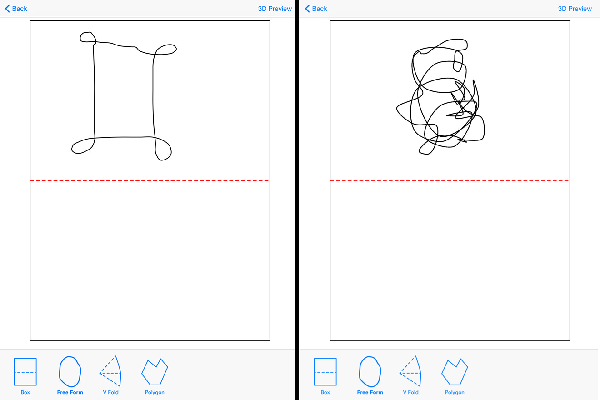
\includegraphics{figures/41_Tech_Tool_Implementation/succeedFailSelfIntersections.pdf}
\caption{Left: a feature with multiple self-intersecting loops, which
our algorithm can repair. Right: a feature with multiple overlapping
intersections, which our algorithm fails to repair.}
\end{figure}
